
%%%%%%%%%%%%%%%%%%%%%%%%%%%%%%%%%%%%%%%%%%%%%%%%%%%%%%%%%%%%%%%%%%%%%%%%%%%%%%%%%%%%%%%
%%%%%%%%%%%%%%%%%%%%%%%%%%%%%%%%%%%%%%%%%%%%%%%%%%%%%%%%%%%%%%%%%%%%%%%%%%%%%%%%%%%%%%%
% 
% This top part of the document is called the 'preamble'.  Modify it with caution!
%
% The real document starts below where it says 'The main document starts here'.

\documentclass[12pt]{article}

\usepackage{amssymb,amsmath,amsthm}
\usepackage[top=1in, bottom=1in, left=1.25in, right=1.25in]{geometry}
\usepackage{fancyhdr}
\usepackage{enumerate}
\usepackage{listings}
\usepackage{graphicx}
\usepackage{float}
\usepackage{multicol}
% Comment the following line to use TeX's default font of Computer Modern.
\usepackage{times,txfonts}
\usepackage{mwe}
\usepackage{caption}
\usepackage{subcaption}





\makeatletter
\renewcommand*\env@matrix[1][*\c@MaxMatrixCols c]{%
  \hskip -\arraycolsep
  \let\@ifnextchar\new@ifnextchar
  \array{#1}}
\makeatother

\newtheoremstyle{homework}% name of the style to be used
  {18pt}% measure of space to leave above the theorem. E.g.: 3pt
  {12pt}% measure of space to leave below the theorem. E.g.: 3pt
  {}% name of font to use in the body of the theorem
  {}% measure of space to indent
  {\bfseries}% name of head font
  {:}% punctuation between head and body
  {2ex}% space after theorem head; " " = normal interword space
  {}% Manually specify head
\theoremstyle{homework} 

% Set up an Exercise environment and a Solution label.
\newtheorem*{exercisecore}{Exercise \@currentlabel}
\newenvironment{exercise}[1]
{\def\@currentlabel{#1}\exercisecore}
{\endexercisecore}

\newcommand{\localhead}[1]{\par\smallskip\noindent\textbf{#1}\nobreak\\}%
\newcommand\solution{\localhead{Solution:}}

%%%%%%%%%%%%%%%%%%%%%%%%%%%%%%%%%%%%%%%%%%%%%%%%%%%%%%%%%%%%%%%%%%%%%%%%
%
% Stuff for getting the name/document date/title across the header
\makeatletter
\RequirePackage{fancyhdr}
\pagestyle{fancy}
\fancyfoot[C]{\ifnum \value{page} > 1\relax\thepage\fi}
\fancyhead[L]{\ifx\@doclabel\@empty\else\@doclabel\fi}
\fancyhead[C]{\ifx\@docdate\@empty\else\@docdate\fi}
\fancyhead[R]{\ifx\@docauthor\@empty\else\@docauthor\fi}
\headheight 15pt

\def\doclabel#1{\gdef\@doclabel{#1}}
\doclabel{Use {\tt\textbackslash doclabel\{MY LABEL\}}.}
\def\docdate#1{\gdef\@docdate{#1}}
\docdate{Use {\tt\textbackslash docdate\{MY DATE\}}.}
\def\docauthor#1{\gdef\@docauthor{#1}}
\docauthor{Use {\tt\textbackslash docauthor\{MY NAME\}}.}
\makeatother

% Shortcuts for blackboard bold number sets (reals, integers, etc.)
\newcommand{\Reals}{\ensuremath{\mathbb R}}
\newcommand{\Nats}{\ensuremath{\mathbb N}}
\newcommand{\Ints}{\ensuremath{\mathbb Z}}
\newcommand{\Rats}{\ensuremath{\mathbb Q}}
\newcommand{\Cplx}{\ensuremath{\mathbb C}}
%% Some equivalents that some people may prefer.
\let\RR\Reals
\let\NN\Nats
\let\II\Ints
\let\CC\Cplx
%%%%%%%%%%%%%%%%%%%%%%%%%%%%%%%%%%%%%%%%%%%%%%%%%%%%%%%%%%%%%%%%%%%%%%%%%%%%%%%%%%%%%%%
%%%%%%%%%%%%%%%%%%%%%%%%%%%%%%%%%%%%%%%%%%%%%%%%%%%%%%%%%%%%%%%%%%%%%%%%%%%%%%%%%%%%%%%
% 
% The main document start here.




%  \textbf{Code:}
%  \begin{center}
%  \lstinputlisting[basicstyle = \footnotesize]{}
%  \end{center}
%  
%  \begin{footnotesize}
%  \begin{verbatim}
%    
%  \end{verbatim}
%  \end{footnotesize}
%  
%  
%  \begin{figure}[H]
%    \begin{center}
%      \caption{}
%    \includegraphics[width = \textwidth]{}
%    \end{center}
%  \end{figure}





% The following commands set up the material that appears in the header.
\doclabel{Stat 605: Exam 2}
\docauthor{Stefano Fochesatto}
\docdate{\today}

\begin{document}

\begin{exercise}{1} Definitions. For each of the following, define the term and stat its importance in statistics (spatial 
  statistics if the term is specific to spatial stats). (I expect 2-3 sentences for each of these, no more.)\\
  \begin{enumerate}
    \item[(a)] Edge effects (for point pattern data)\\
    \solution Edge effects, as the name suggests are biases in our point pattern analysis that arise from having a closed study region. An important example comes when we 
    use nearest neighbor distances as a test for CSR. We find that event along the edge of a study region will ignore nearest neighbors that might be found outside of the study region, resulting in greater distances an biasing our results. 

    \vspace{.15in} 
    \item[(b)] CSR (complete spatial randomness)\\
    \solution CSR is a measure used to recognize the randomness in spatial region. Formally we define a spatial process as exhibiting CSR to have the property that 
    the number of points in any given sub region $U_i$ follows a Poisson distribution (Poisson($\gamma_i$)) where $\gamma_i = \lambda \times \text{ $area_{U_i}$} $, 
    additionally the number of points in non-overlapping regions are independent. Note that CSR is synonymous with a homogenous Poisson Process. 
    \vspace{.15in} 
    \item[(c)] Monte Carlo tests (also, why are they so useful when working with point pattern data?)\\
    \solution As the name suggests Monte Carlo tests rely on performing repeated random simulations of data to compute the empirical distribution of a desired test statistic with the goal estimating a p-value for 
    the test statistic of our original data. The application to point pattern data is substantial specifically when testing if
    our data exhibits CSR. We saw Monte Carlo tests used to simulate CSR k-functions, nearest neighbor distances, and quadrat counts. As a result of using the empirical distribution these Monte Carlo tests
    provide more relaxed assumptions when compared to their original tests; for example the Monte Carlo quadrat test does not assume that the index of dispersion(test statistic) is chi-squared distributed, 
    this distribution is simulated instead. 
  \end{enumerate} 
\end{exercise}
\newpage


\begin{exercise}{2} We model CSR using a spatial Poisson process (for point pattern data). Consider a rectangular region $R$
  with $0 \geq x \geq 3$ and $0 \geq y \geq 2$.\\
  \begin{enumerate}
    \item[(a)] If the intensity for a (homogenous) Poisson process in this region is given by $\lambda(x, y) = 1.4,$\\ 
    \begin{enumerate}
      \item[i.] What is the distribution of $N(R),$ the number of events in the region?\\
      \solution As discussed in the previous problem we know that the distribution of $N(R)$ is Poisson($\gamma$) where $\gamma = \lambda \text{R}$. Doing so we find that, 
      \begin{equation*}
        N(R) \sim \text{Poisson}(1.4(3)(2)) = \text{Poisson}(8.4). 
      \end{equation*}
      \vspace{.15in}
      \item[ii.] Find $P(N(R) = 12),$ the probability that there are 12 events in the region.\\
      \solution Plugging our values into the Poisson distribution we get the following, 
      \begin{equation*}
        P(N(R) = 12) = \dfrac{8.4^{12}}{12!}e^{-8.4} = 0.058.
      \end{equation*}
      \vspace{.15in}
    \end{enumerate} 

    \item[(b)] If the intensity of the inhomogeneous Poisson process in this region is $\lambda(x, y) = x + y$, \\
    \begin{enumerate}
      \item[i.] Calculate $\gamma = \iint_R \lambda(x, y) dx dy$\\
      \solution Setting up the integral and then solving we get the following, 
      \begin{align*}
        \gamma &= \int_0^2 \int_0^3 x + y dxdy,\\
         &= \int_0^2 [\dfrac{x^2}{2} + xy]_0^3 dy,\\
         &= \int_0^2 \dfrac{9}{2} + 3y dy,\\
         &=  \dfrac{3y^2}{2} + \dfrac{9}{2}y |_0^2,\\
         &=  15.
      \end{align*}
      \vspace{.15in}
      \item[ii.] Find the distribution of $N(R)$\\
      \solution For inhomogeneous Poisson processes we know that $N(R)$ is still Poisson distributed, in this case the $\gamma$ parameter is computed 
      with the previous integral and for any sub regions we change the bounds of integration. Therefore we get the following distribution when $\lambda(x, y) = x + y$.\\
      \begin{equation*}
        N(R) \sim \text{Poisson}(15).
      \end{equation*}
      \vspace{.15in}
     \item[iii.] What is the expected number of events in the region R?\\
     \solution By definition a random variable $X$ which follows a Poisson distribution with rate parameter $\gamma$ has the property that, $\gamma = E(X) = Var(X)$. Therefore we know that, 
     \begin{equation*}
       E(N(R)) = 15. 
     \end{equation*}
    \end{enumerate} 
  \end{enumerate}
\end{exercise}
\vspace{.5in}




\begin{exercise}{3} For each of the following traceplots from a Bayesian analysis of geostatistical spatial data,
  \begin{itemize}
    \item Identify whether the traceplot indicates that convergence has occurred
    \item State whether we should omit iterations as burn-in (if so, indicate how much)
    \item State whether we should use narrower or wider Metropolis proposals (or do they already seem appropriate); If narrower, why will making them 
    narrower help? If wider, why will making them wider help?
    \item Do you think we should run our MCMC for more iterations?
  \end{itemize}
  \begin{enumerate}
    \item[a.] 
    \solution The following traceplot seems typical of a non-negative parameter since it has a floor at zero, plotting log(theta) might fix that. 
    We can see that at around 500 iterations there is good convergence outside of the minor spikes here and there. 
    The plot does show iterations from 0 to about 100 that might need to be omitted as burn-in. The shape of the trace plot does not indicate to me that we need to adjust the 
    Metropolis proposal size (neither baby steps or big blocks; very grassy). Running MCMC for more iterations might be helpful to really confirm the convergence of the parameter but does not seem necessary. 
    \begin{figure}[H]
      \begin{center}
      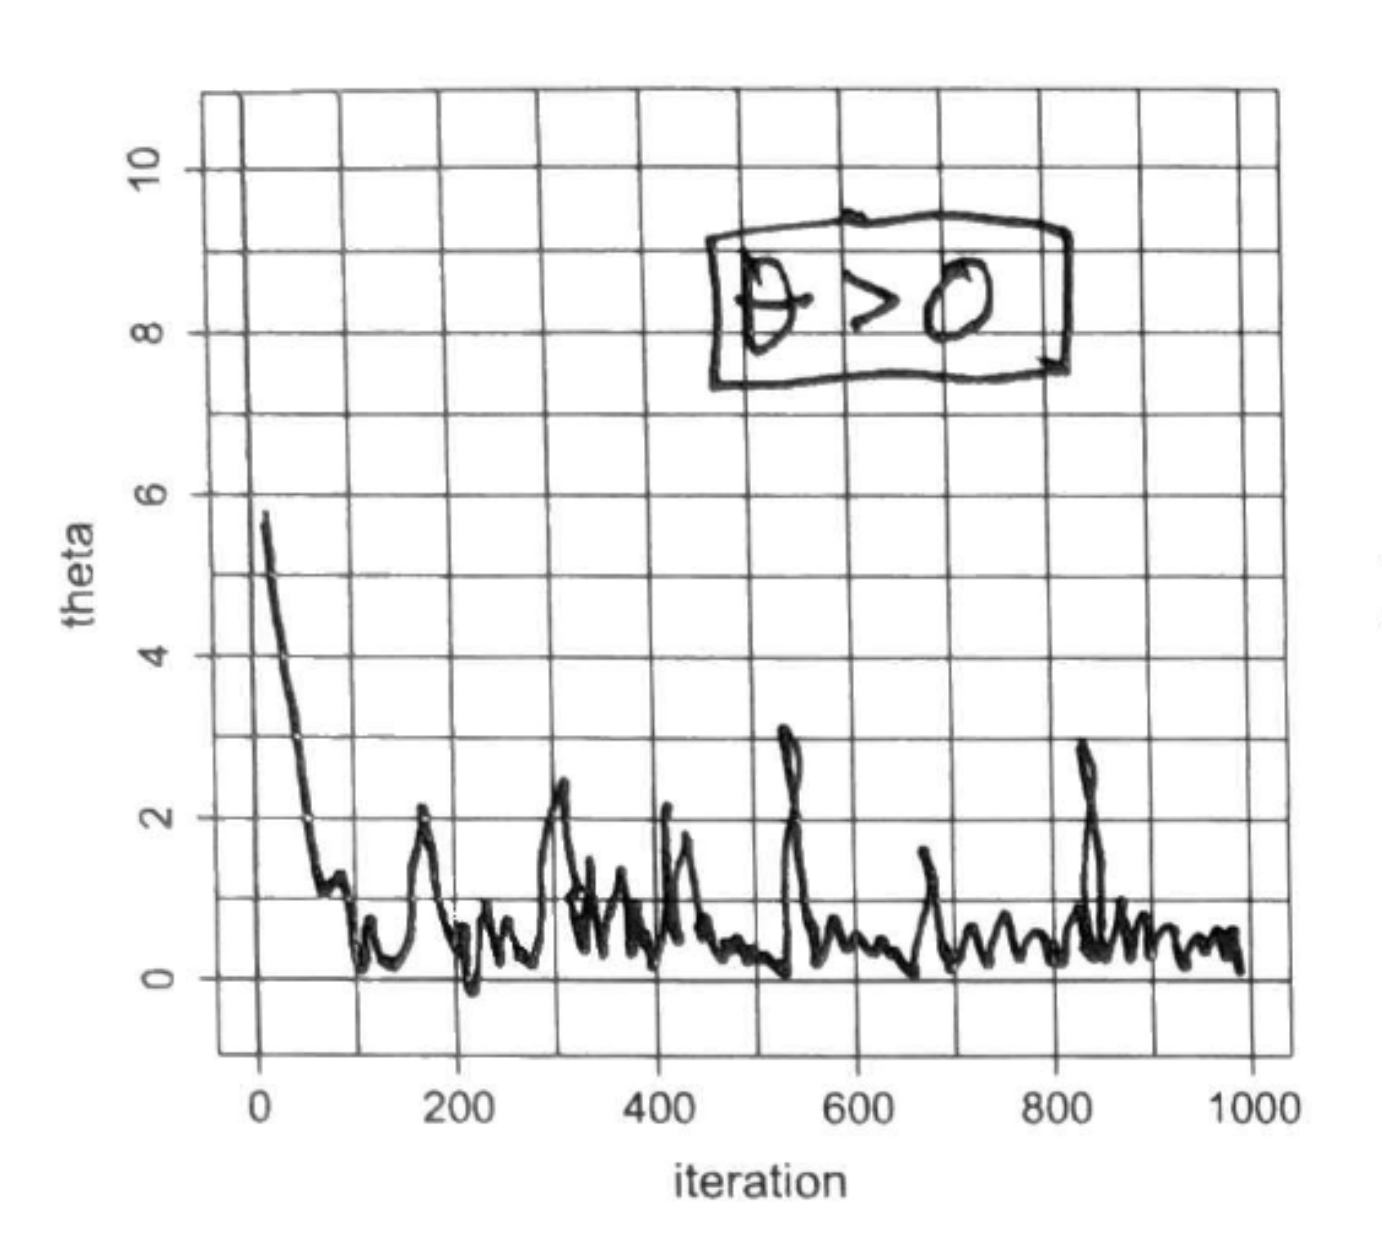
\includegraphics[width = .6\textwidth]{1traceplot.png}
      \end{center}
    \end{figure}
    \item[b.]
    \solution This trace plot seems to be exhibiting a ceiling on the values at around 5 and does not indicate convergence. To fix this we would want to adjust the prior for the 
    $\theta$ parameter to include a greater range of values. Burn-in looks about the same as the previous plot, we could omit iterations 1 to about 100. 
    The shape again does not indicate that the Metropolis proposal size needs adjusting. Depending on the trace plot for the adjusted prior we might need more iterations. 
    \begin{figure}[H]
      \begin{center}
      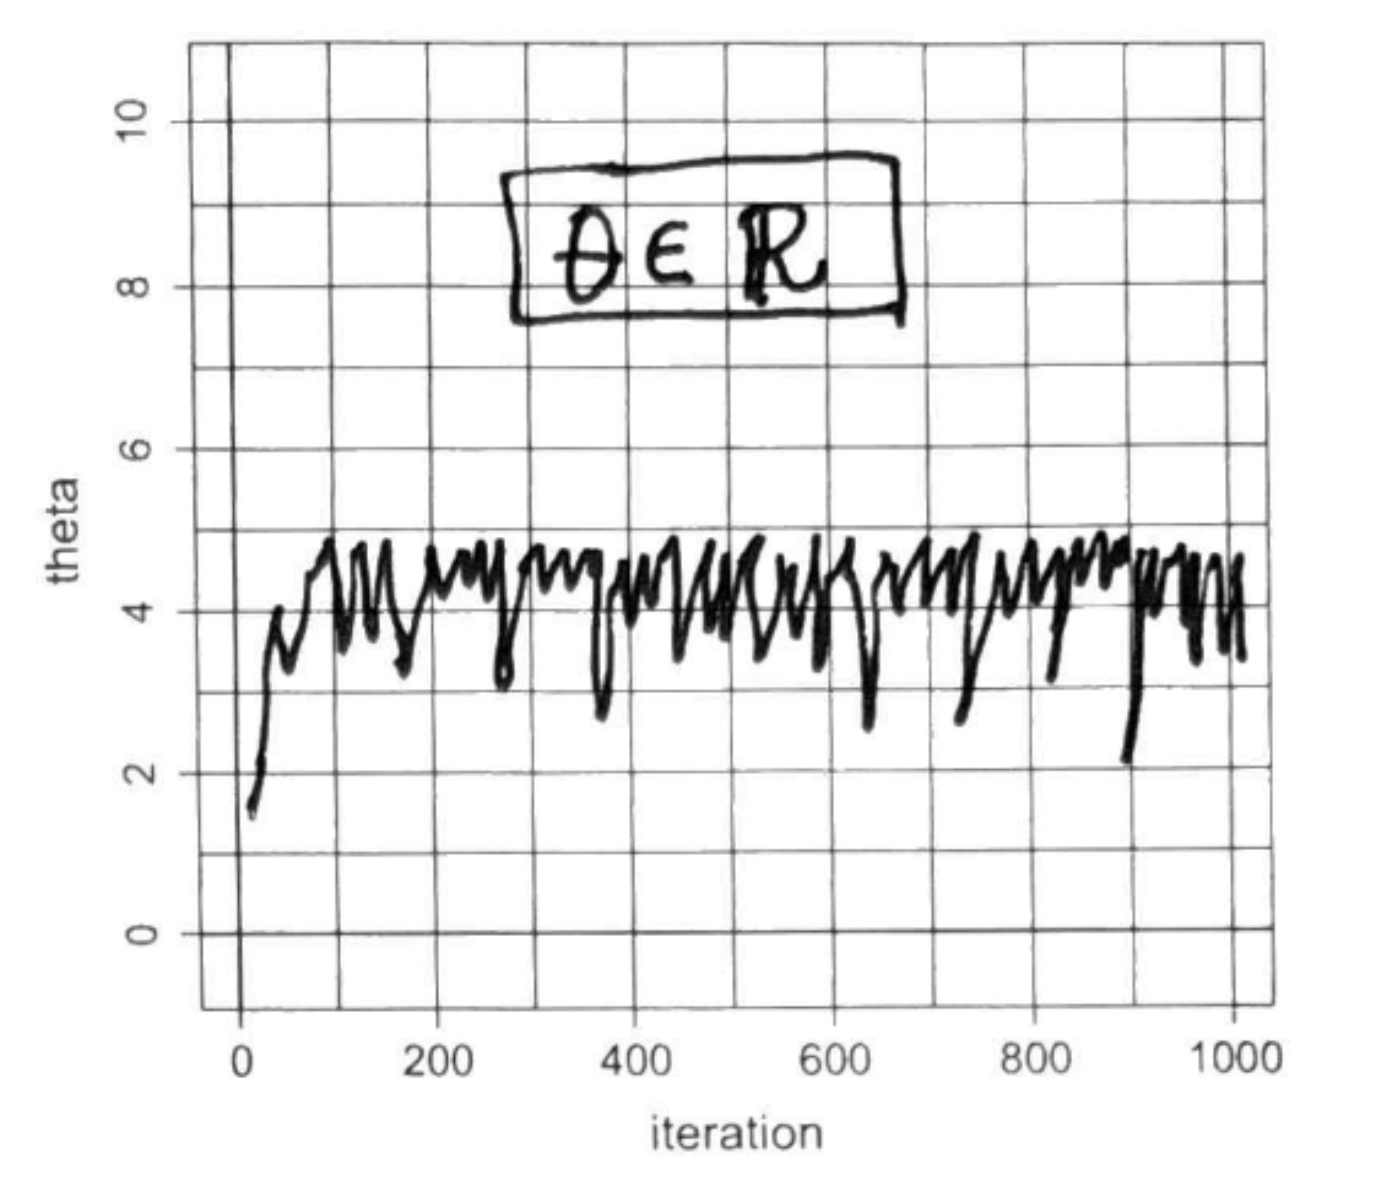
\includegraphics[width = .6\textwidth]{2traceplot.png}
      \end{center}
    \end{figure}
    \item[c.] 
    \solution This trace plot looks to converge at around a value of 4. We can see very clearly that iterations 0 to around 500 should be omitted as burn-in. 
    Ignoring the burn-in iterations the plot does not suggest that the Metropolis proposal size should be adjusted. I don't think more iterations are necessary, since the plot seems to show convergence.
    \begin{figure}[H]
      \begin{center}
      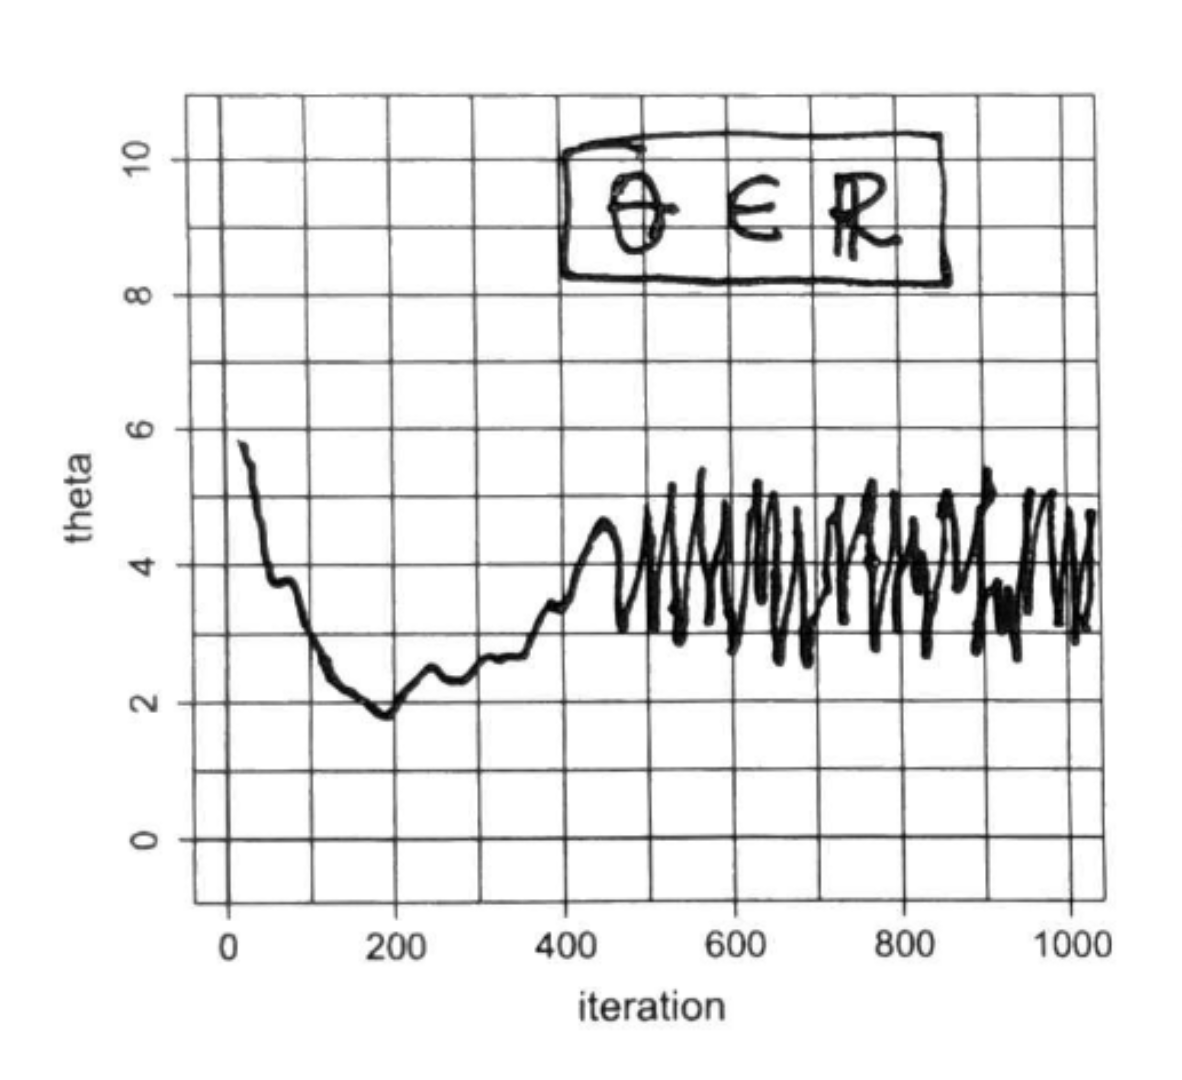
\includegraphics[width = .6\textwidth]{Traceplot3.png}
      \end{center}
    \end{figure} 

    \item[d.] 
    \solution The following trace plot does not exhibit convergence. To address this we could run MCMC for more iterations (in class you've suggested 5000 iterations), or we could adjust the Metropolis proposal size and make it larger. 
    We are seeing slow convergence because out Metropolis proposals are too small and it's taking many many iterations to explore to explore the shape of the posterior distribution. 
    \begin{figure}[H]
      \begin{center}
      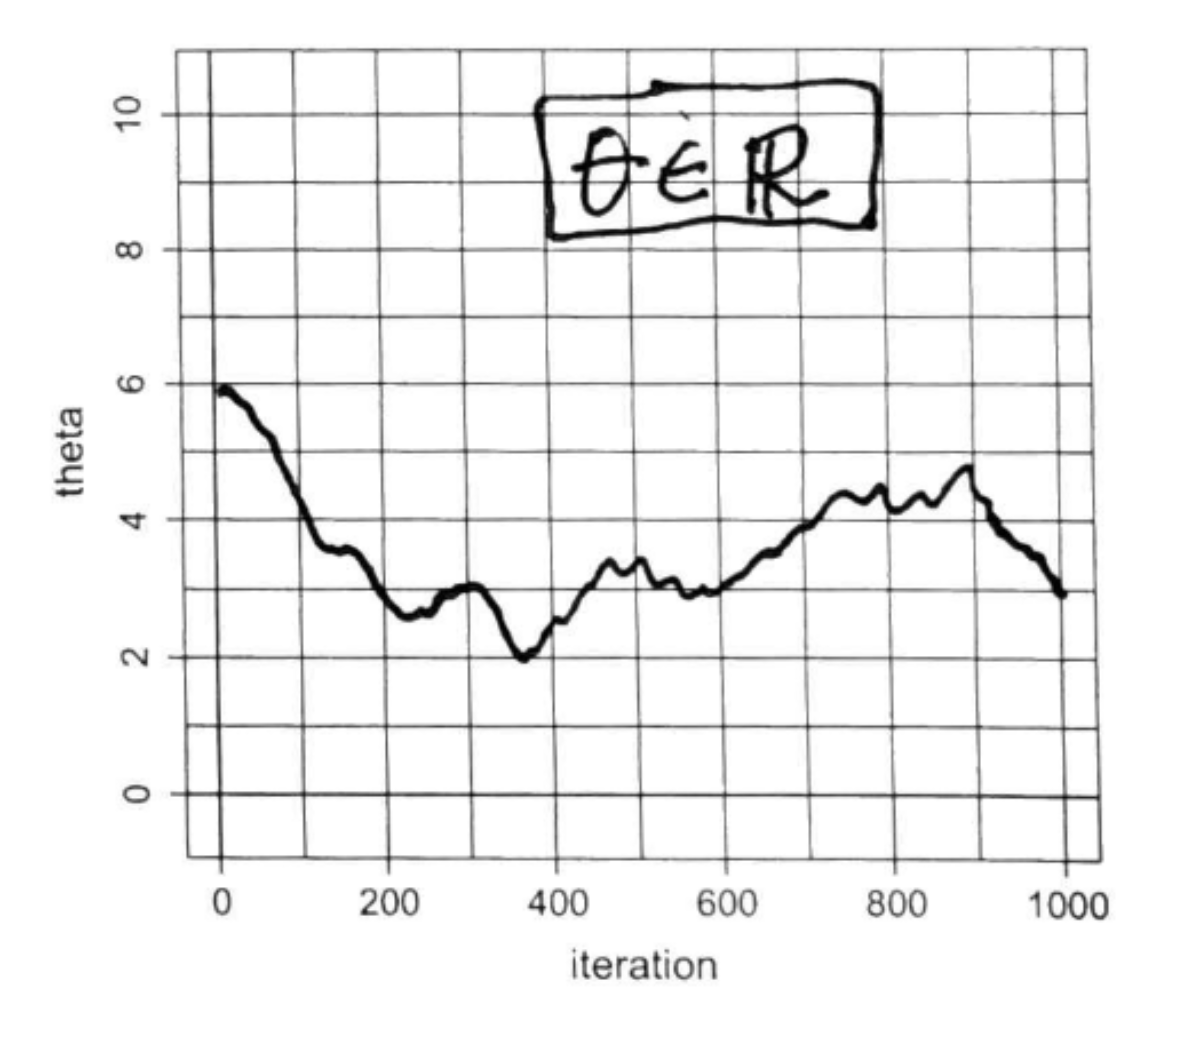
\includegraphics[width = .6\textwidth]{Traceplot4.png}
      \end{center}
    \end{figure} 
  \end{enumerate}
\end{exercise}

\vspace{.5in}

\begin{exercise}{4} I wish to conduct a formal test for CSR using $m = 11$ randomly selected quadrats. The counts are:
  \begin{equation*}
    \{5,6,8,5,6,5,6,5,6,6,6\}
  \end{equation*}
  \begin{enumerate}
    \item[a.] I suspect from looking at these data that there is some evidence of regularity. Why? What is it about these data that seems at face value to 
    be consistent with regularity? What would we expect to see (and why) if there were clustering?\\
    \solution This data suggests regularity because it exhibits very low variance relative to the mean so in each quadrat we are capturing a similar number of points. Recall that for CSR data we expect the quadrat count to follow a Poisson distribution and therefore the estimated mean and variance should be similar. 
    When the data is clustered we expect the estimated variance to be a lot larger than the estimated mean simply because in some cases quadrats will capture entire clusters and others will capture no data.\\
    \vspace{.15in}


    \item[b.] For these data, the sample mean is 5.82 and the sample variance is .764. Carry out a hypothesis test of 
    $H_0: CSR$ versus $H_a: \text{regularity}$, using $\alpha = .05$. Be sure to calculate p-values. Be sure to state your conclusions in layman's terms.\\
    \solution Conducting a test for regularity using quadrat data we must first compute our test statistic (index of dispersion). 
    \begin{equation*}
      I = \dfrac{(m - 1)s^2}{\bar{y}} = \dfrac{(11 - 1).764}{5.82} = 1.313. 
    \end{equation*}
    Recall that $I \approx \chi^2(m-1)$ and that for conducting a regularity test we compute the p-value using the left tail of the $\chi^2$ distribution. Doing so in r we get the following, 
    \textbf{Code:}
    \begin{center}
    \lstinputlisting[basicstyle = \footnotesize]{r1.txt}
    \end{center}
    With a p-value of 0.0005906407 at the $\alpha = .05$ level we reject the null and conclude that the data is exhibiting some regularity. 
  \end{enumerate}
\end{exercise}
\vspace{.5in}




\begin{exercise}{5} Use the plots below to answer the following questions about the locationa of 99 people sitting in Gordon Park having a picnic on a sunny day. There are two holes 
  in the region. Distances are in meters (This is gordon data in the spatstat package.)\\
  \begin{figure}[H]
    \begin{center}
    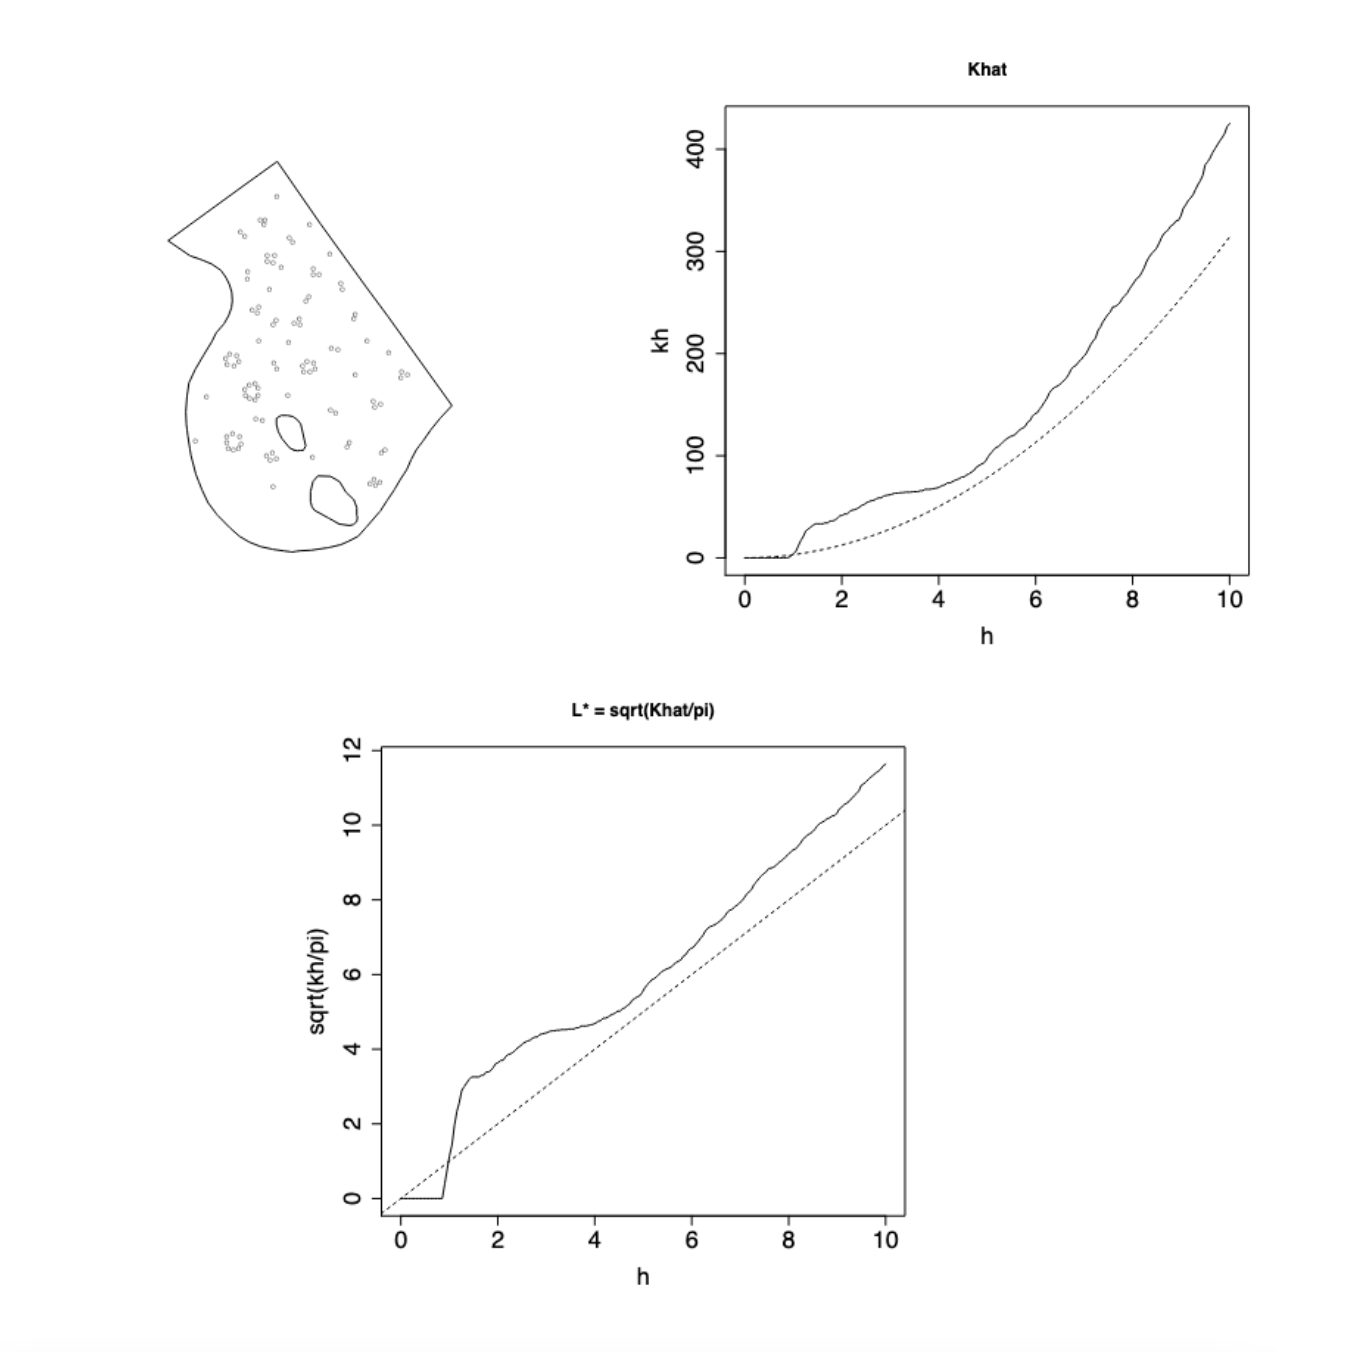
\includegraphics[width = .6\textwidth]{kfunction.png}
    \end{center}
  \end{figure} 








  \begin{enumerate}
    \item[a] The first plot shows the locations of the picnickers. Comment on the plot; any unusual features? Do you see any strong evidence of clustering or regularity.\\
    \solution We can see that at a low scale there is definitely evidence of clustering, but zooming out to a larger scale it looks like we find that the clusters are regularly spaced. This idea definitely makes sense 
    from a physical perspective. I'd imagine picnickers, begin to identify that they need to be regularly spaced as the park reaches capacity, in order to accommodate everybody.  
    \vspace{.15in}
    
    
    \item[b] What is the definition of 'K-function'?\\
    \solution The K-function is an extension of the nearest neighbor statistic, and it's designed to identify clustering or regularity at different scales. Formally we define a K-function as 
    the expected number of objects within a distance $h$ of a randomly selected event divided by the density $D$ of the region, 
    \begin{equation*}
      K(h) = \dfrac{1}{D} \mathbb{E}\left(\text{count of objects within distance h of a random event.}\right)
    \end{equation*}
    We compute the estimated K-function with the following,  
    \begin{equation*}
      \hat{K}(h) = \dfrac{1}{\bar{D}} \left(\dfrac{1}{n} \sum_{i = 1}^n N(s_i, h)\right)
    \end{equation*}
    Where $\bar{D}$ is the estimated density over our region of interest, and $N(s_i, h)$ is the count of events inside a circle of with radius $h$ and center $s_i$.
    \vspace{.15in}
    
    
    \item[c] The second plot shows an estimated K-Function (solid) line along with the K-functions corresponds to CSR (dashed curve); the 3rd plot shows $L^* = \sqrt{K/\pi}$. Discuss 
    the features of these plots is there evidence of regularity or clustering at any scale? How can you tell? What explains the initial flat spot in the plot (h < 1ms)? What explains the jump in the plot just to the right of 
    $h = 1ms$? What are you looking for in these plots?\\
    \solution Interestingly the plots for the estimated K-function go against our interpretation from part b. We find that on both plots (more evident on the third plot) that at a small scale the expected number of events is lower than 
    CSR K- function which is indicative of regularity and at larger scales we are seeing many more events than CSR K-function which indicates clustering. The initial flat spot can be explained as a minimum distance between picnickers, clearly if there 
    is a minimum distance between events the K-function will have a value of zero for that initial range, furthermore it suggests to me that inside of the clusters the picnickers are regularly spaced. The large jump for $h > 1$ comes from the sizes of the individual clusters, 
    we can see that a majority of them have around 2 to 4 picnickers. Generally we want to see where the estimated K-function differs from the CSR K-function. If it is above or below the CSR K-Function and at what value of $h$ we see change.
    \vspace{.15in}

  \end{enumerate} 
  
\end{exercise}




\begin{exercise}{6} For the picnic data on the previous page, I use a Monte Carlo test using the
  test statistic
  \begin{equation*}
    A = 2\sqrt{\lambda} \bar{W}
  \end{equation*}
  where $W = \text{distance}$ from a randomly selected event to another event.
(I use the Monte Carlo test because I am worried about edge effects.)
Use the R output below to test H0\: CSR versus Ha\: clustering. What is the
value of my test statistic? What is the p-value? What is your conclusion?




\begin{footnotesize}
\begin{verbatim}
> # find all nearest event distances:
> W <- nndistG( cbind(gordon2$x,gordon2$y) )$dists
> W[1:3]
[1] 4.940166 1.109053 1.141082
> min(W)
[1] 0.854578
> ( n.tot <- length(gordon2$x) )
[1] 99
> ( n.in.SRS <- round(n.tot/10) )
[1] 10
> # Here’s the sample of events I’ll use for the test:
> some.W <- sample(W, size=n.in.SRS, replace=FALSE)
> foo <- gordon2$window$bdry[[1]]
> ( area.of.park <- areapl(cbind(foo$x,foo$y)) )
[1] 2244.576
> ( lambda.hat <- n.tot / area.of.park )
[1] 0.04410633
> ( AA <- 2*sqrt(lambda.hat)*mean(some.W) )
[1] 0.6907354
> n.sims <- 2000
> A.results <- rep(NA,n.sims)
> for( i in 1:n.sims ) {
+ my.sim.data <- csr( mypoly, npoints=n.tot)
+ all.W <- nndistG( my.sim.data )$dists
+ some.W <- sample( all.W, size=n.in.SRS, replace=FALSE)
+ A.results[i] <- 2*sqrt(lambda.hat)*mean(some.W)
+ }
> median(A.results)
[1] 1.038397
> rank( c(AA,A.results) )[1]
[1] 37
\end{verbatim}
\end{footnotesize}

\solution The computed test statistic is the variable AA. The R output says the test statistic has a value of 0.6907354. 
The simulated empirical distribution function for the $A$ test statistic results in a median of 1.038397. Test statistics similar to this 
value should represent CSR data. Having a test statistic smaller than this means that generally the nearest neighbor is closer than that of CSR data which 
suggests clustered data. The final command rank() command tells us where our original data's test statistic lies in relation to the rest; It's the 37 th smallest. 
We can use this to compute the p-value, since we have a total of 2001 test statistics our p-value for the clustering test is given by, 
\begin{equation*}
  p-value = \dfrac{36}{2001} = .01799.
\end{equation*}
With an alpha of $.05$ we would reject the null and conclude that our data are clustered.   
\end{exercise}
\vspace{.15in}




\begin{exercise}{7} The data set “exam2data.txt”, which is posted on Canvas, 
  contains planar point data consisting of 284 events. Please download the data and\:
  \begin{enumerate}
    \item[a]Plot the data (include with your solutions, as usual)\\
    \solution Importing the data and calling plot() we get the following figure. It does not seem to me that it is clustered or regularly spaced. 
    \begin{figure}[H]
      \begin{center}
      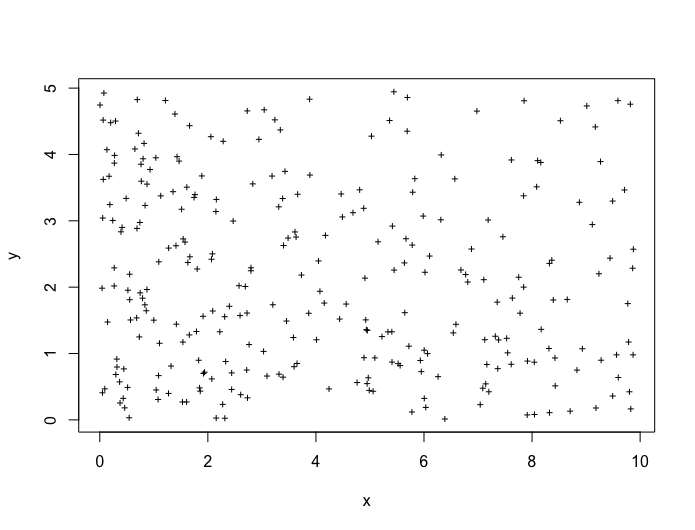
\includegraphics[width = .9\textwidth]{Rplot.png}
      \end{center}
    \end{figure} 
    \textbf{Code:}
    \begin{center}
    \lstinputlisting[basicstyle = \footnotesize]{r2.txt}
    \end{center}
    \vspace{.15in}
    
    \item[b] Does it appear consistent with CSR? Conduct three tests for CSR: a 
    suitable quadrat test with perhaps 18 grid cells; a Monte Carlo test using a
    measure of event-event distance (e.g. the test that uses W, and a Monte
    Carlo test using a K-function). State your conclusions, and be sure to
    summarize in a table (test statistic and p-values?), and provide suitable
    plots where appropriate.\\
    \solution Conducting a two sided quadrat test on 18 grid cells we get test statistic of 60.155 and p-value of 1.982e-06. With an $\alpha = .05$ significance 
    level we would reject the null and conclude that the data does not appear consistent with CSR. 
    \begin{figure}[H]
      \begin{center}
      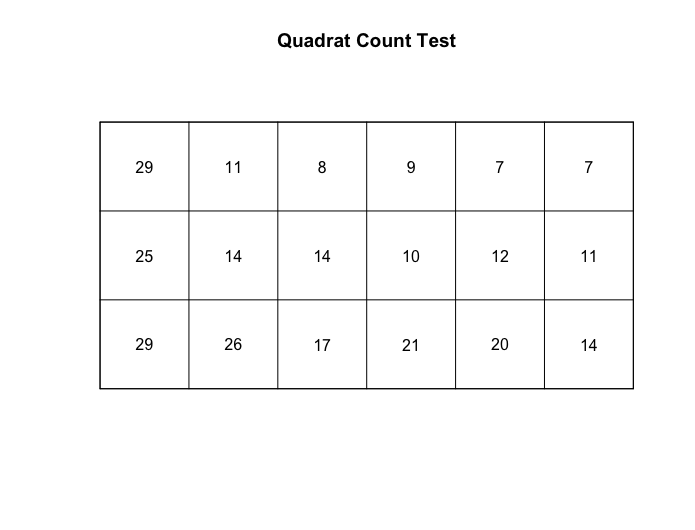
\includegraphics[width = .9\textwidth]{Rplot01.png}
      \end{center}
    \end{figure} 
    \textbf{Code:}
    \begin{center}
    \lstinputlisting[basicstyle = \footnotesize]{r3.txt}
    \end{center}

    Conducting a Monte Carlo test using a K-function we get the following envelope, and we get a p-value of 0.05666667. With an $\alpha = .05$ significance level we would fail to 
    reject the null, that the data are consistent with CSR. P-value was computed similarly to the previous problem, our data was rank 284 out of 300 we get the following, 
    \begin{equation*}
      p-value = \dfrac{300 - 284 + 1}{300} = 0.05666.
    \end{equation*}
    The envelope figures show that the estimated k-function for our data are mostly within the margins of our simulated data, which agrees with the results of our test. 

    \begin{figure}[H]
      \begin{center}
      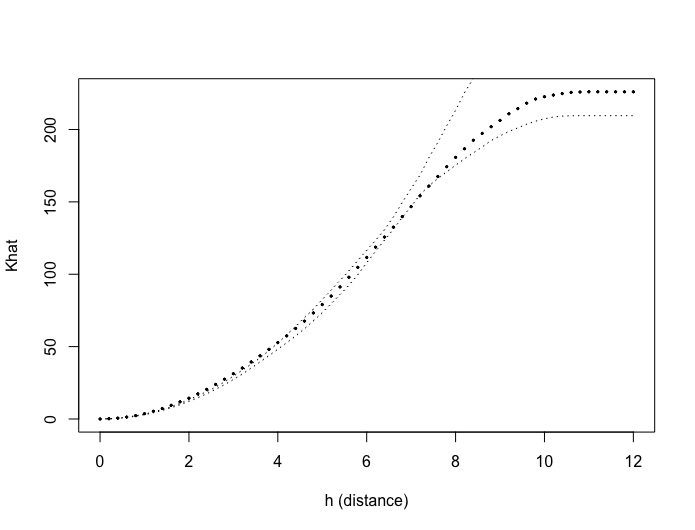
\includegraphics[width = .9\textwidth]{Rplot03.png}
      \end{center}
    \end{figure} 

    \begin{figure}[H]
      \begin{center}
      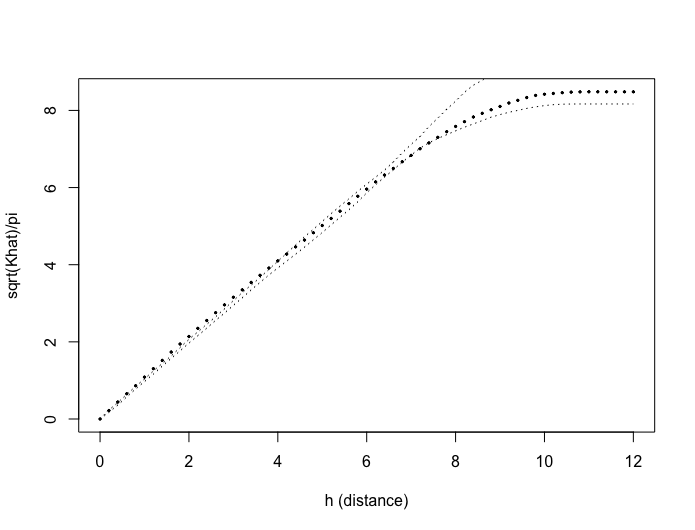
\includegraphics[width = .9\textwidth]{Rplot04.png}
      \end{center}
    \end{figure} 



    \begin{figure}[H]
      \begin{center}
      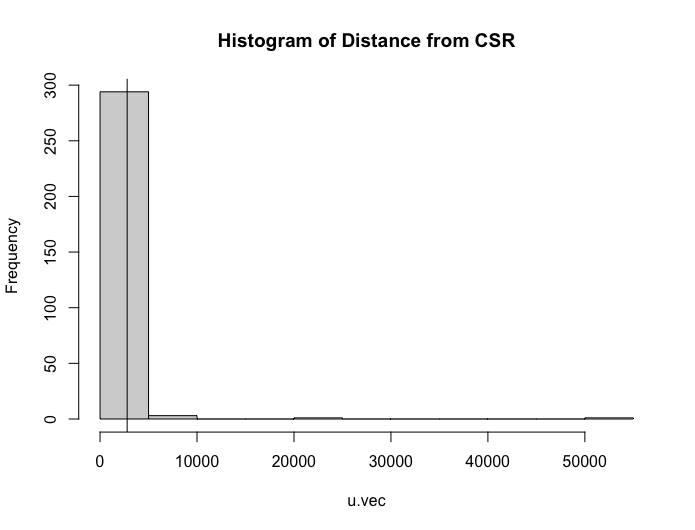
\includegraphics[width = .9\textwidth]{Rplot06.png}
      \end{center}
    \end{figure} 



    \textbf{Code:}
    \begin{center}
    \lstinputlisting[basicstyle = \footnotesize]{r4.txt}
    \end{center}
    
    Conducting a distance based montecarlo test using nearest neighbor distances (W) and the $A = 2\sqrt(\lambda)\bar{W}$ test statistic, our data achived a rank of 890 out of 2001. 
    Computing the two sided p-value we get the following, 
    \begin{equation*}
      p-value = \dfrac{2001 - 890 + 1}{2001} = .555.
    \end{equation*}


    \textbf{Code:}
    \begin{center}
    \lstinputlisting[basicstyle = \footnotesize]{r6.txt}
    \end{center}
    \vspace{.15in}




    \item[c] Regardless of what are the conclusions of part (b), fit models for an in-
    homogeneous Poisson process, including an intercept-only model, models
    containing first and second order terms (including possible interaction).
    Select the best model using AIC. Provide a table that summarizes AIC for
    each of the models you examined.
    What is your winning model?\\
    \solution Fitting each of the four models: Intercept, first order, second order no interaction, and full second order using the ppm function we get the following AIC table. 

    \begin{center}
      \begin{tabular}{|c||c| }
        \hline
        Model & AIC \\
        \hline 
        \hline
        Intercept& -416.5883 \\
        First Order& -457.5101  \\
        Second Order No Interaction& -460.5883   \\
        Full Second Order& -462.3144 \\
        \hline
       \end{tabular}
      \end{center}

    \textbf{Code:}
    \begin{center}
    \lstinputlisting[basicstyle = \footnotesize]{r7.txt}
    \end{center}
    \vspace{.15in}



      Of each of the models we can see that the Full Second Order model achieves the lowest AIC. 









    \vspace{.15in}


    \item[d] State the estimated intensity at $s=(1.0,1.0)$ for your winning model.\\
    \solution Recall that ppm fits a function for the log of the intensity, and since we are finding the intentsity at point (1,1)
    all we have to do is take the sum of the coefficients and raise it to the exp(). Doing so we get $\lambda = 10.50405$. \\
    \textbf{Code:}
    \begin{center}
    \lstinputlisting[basicstyle = \footnotesize]{r8.txt}
    \end{center}
  \end{enumerate}
  
\end{exercise}
\vspace{.5in}

\begin{exercise}{8} Poisson Cluster Processes. 
  \begin{enumerate}
    \item[a] Fit a Poisson cluster process model to the redwood3 data set, which is
    built into the spatstat package.\\
    \begin{enumerate}
      \item[i] How many events are there? Estimate the density of the events (i.e.
      number per unit area; state the units!)\\
      \solution There 62 events in the redwood3 data set which can be found by calling length on redwood3\$x. We can see that the redwood3\$window
      object plots the region in a 1x1 square. With no further information we can estimate the density to be 62 events per unit area. 
      \vspace{.15in}


      \item[ii] What are the estimates of s2 and $\rho$? What do these represent?\\ 
      \solution Fitting the model we get the following s2 and $\rho$. Interpreting these values we know that $\rho$ is an estimate for parent intensity, 
      so we would say that there are 32.08 parent events per unit area. s2 is the variance of the bivariate normal distribution which fits spread of the offspring.\\
      
      \textbf{Code:}
      \begin{center}
      \lstinputlisting[basicstyle = \footnotesize]{r9.txt}
      \end{center}
      \vspace{.15in}


      \item[iii] How might we estimate the number of “parents” for the clusters? Will
      we be very sure of this value? (What distribution are the number of
      parents following?)\\
      \solution By definition of a Poisson Cluster Process we know that the parent events follow a Poisson process with a constant intensity $\rho$. Using our estimated $\rho$ we 
      can say that there are around 32 parents since this region has area 1. Since these events follow a Poisson distribution, which has the same variance as $\rho$ for a region this small we cannot be sure of this value at all. 
      A confidence interval for the expected count comes out to about (21,43).
      \vspace{.15in}

      \item[iv] How might we estimate the number of “offspring” per cluster? (Esti-
      mate this!)\\
      \solution We know that there are about $\rho \times \text{area}$ as many parents. Since we know the total number of events in the region we can subtract from that to get the number of offspring. 
      Doing so with an estimated 32 parents we get 30 offspring. By division we get $30/32 \approx .9$ offspring per parent. 
    \end{enumerate}



    \item[b] Repeat (a) for the data set in problem 7. These data aren't clustered. Do
    you see anything in the computer output from pcp that reflects this? Comment briefly. (This last question is somewhat open-ended, and there may
    be nothing very striking about the output, other than that you might've
    expected very unusual, given that the data are so obviously not clustered.)\\
    \solution Running the model and looking at the summary report we get a value of 0.4824805, for our estimated $\rho$ and $0.699637$ for our estimated s2. This data spans a larger region, and from the 
    looks of it the model is finding very few parents. Multiplying $\rho$ by the are of the region we get an approximate 25 parent events, which means that there are approximately 259 offspring events. Nothing from the 
    summary output screams to me that the data is not clustered. I would think that if it were maybe there would be more parents, and a smaller s2 value, meaning more tightly grouped offspring. 


    \textbf{Code:}
    \begin{center}
    \lstinputlisting[basicstyle = \footnotesize]{r10.txt}
    \end{center}
    \vspace{.15in}
  \end{enumerate}
\end{exercise}

\newpage



\begin{figure}[H]
  \begin{center}
  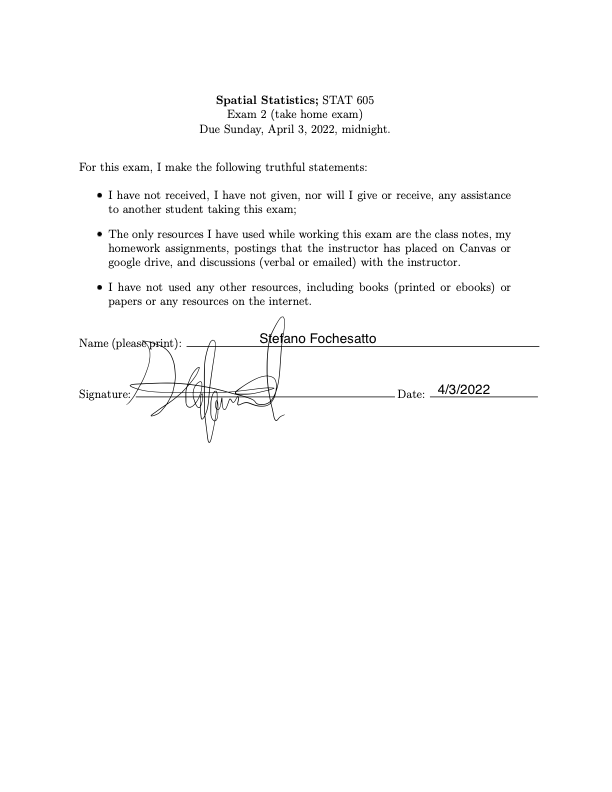
\includegraphics[width = \textwidth]{SignaturePage.png}
  \end{center}
\end{figure} 




\end{document}


















